% Options for packages loaded elsewhere
\PassOptionsToPackage{unicode}{hyperref}
\PassOptionsToPackage{hyphens}{url}
\PassOptionsToPackage{dvipsnames,svgnames,x11names}{xcolor}
%
\documentclass[
]{article}

\usepackage{amsmath,amssymb}
\usepackage{iftex}
\ifPDFTeX
  \usepackage[T1]{fontenc}
  \usepackage[utf8]{inputenc}
  \usepackage{textcomp} % provide euro and other symbols
\else % if luatex or xetex
  \usepackage{unicode-math}
  \defaultfontfeatures{Scale=MatchLowercase}
  \defaultfontfeatures[\rmfamily]{Ligatures=TeX,Scale=1}
\fi
\usepackage{lmodern}
\ifPDFTeX\else  
    % xetex/luatex font selection
    \setmainfont[]{Latin Modern Roman}
  \setmathfont[]{Latin Modern Math}
\fi
% Use upquote if available, for straight quotes in verbatim environments
\IfFileExists{upquote.sty}{\usepackage{upquote}}{}
\IfFileExists{microtype.sty}{% use microtype if available
  \usepackage[]{microtype}
  \UseMicrotypeSet[protrusion]{basicmath} % disable protrusion for tt fonts
}{}
\makeatletter
\@ifundefined{KOMAClassName}{% if non-KOMA class
  \IfFileExists{parskip.sty}{%
    \usepackage{parskip}
  }{% else
    \setlength{\parindent}{0pt}
    \setlength{\parskip}{6pt plus 2pt minus 1pt}}
}{% if KOMA class
  \KOMAoptions{parskip=half}}
\makeatother
\usepackage{xcolor}
\setlength{\emergencystretch}{3em} % prevent overfull lines
\setcounter{secnumdepth}{5}
% Make \paragraph and \subparagraph free-standing
\makeatletter
\ifx\paragraph\undefined\else
  \let\oldparagraph\paragraph
  \renewcommand{\paragraph}{
    \@ifstar
      \xxxParagraphStar
      \xxxParagraphNoStar
  }
  \newcommand{\xxxParagraphStar}[1]{\oldparagraph*{#1}\mbox{}}
  \newcommand{\xxxParagraphNoStar}[1]{\oldparagraph{#1}\mbox{}}
\fi
\ifx\subparagraph\undefined\else
  \let\oldsubparagraph\subparagraph
  \renewcommand{\subparagraph}{
    \@ifstar
      \xxxSubParagraphStar
      \xxxSubParagraphNoStar
  }
  \newcommand{\xxxSubParagraphStar}[1]{\oldsubparagraph*{#1}\mbox{}}
  \newcommand{\xxxSubParagraphNoStar}[1]{\oldsubparagraph{#1}\mbox{}}
\fi
\makeatother


\providecommand{\tightlist}{%
  \setlength{\itemsep}{0pt}\setlength{\parskip}{0pt}}\usepackage{longtable,booktabs,array}
\usepackage{calc} % for calculating minipage widths
% Correct order of tables after \paragraph or \subparagraph
\usepackage{etoolbox}
\makeatletter
\patchcmd\longtable{\par}{\if@noskipsec\mbox{}\fi\par}{}{}
\makeatother
% Allow footnotes in longtable head/foot
\IfFileExists{footnotehyper.sty}{\usepackage{footnotehyper}}{\usepackage{footnote}}
\makesavenoteenv{longtable}
\usepackage{graphicx}
\makeatletter
\def\maxwidth{\ifdim\Gin@nat@width>\linewidth\linewidth\else\Gin@nat@width\fi}
\def\maxheight{\ifdim\Gin@nat@height>\textheight\textheight\else\Gin@nat@height\fi}
\makeatother
% Scale images if necessary, so that they will not overflow the page
% margins by default, and it is still possible to overwrite the defaults
% using explicit options in \includegraphics[width, height, ...]{}
\setkeys{Gin}{width=\maxwidth,height=\maxheight,keepaspectratio}
% Set default figure placement to htbp
\makeatletter
\def\fps@figure{htbp}
\makeatother
% definitions for citeproc citations
\NewDocumentCommand\citeproctext{}{}
\NewDocumentCommand\citeproc{mm}{%
  \begingroup\def\citeproctext{#2}\cite{#1}\endgroup}
\makeatletter
 % allow citations to break across lines
 \let\@cite@ofmt\@firstofone
 % avoid brackets around text for \cite:
 \def\@biblabel#1{}
 \def\@cite#1#2{{#1\if@tempswa , #2\fi}}
\makeatother
\newlength{\cslhangindent}
\setlength{\cslhangindent}{1.5em}
\newlength{\csllabelwidth}
\setlength{\csllabelwidth}{3em}
\newenvironment{CSLReferences}[2] % #1 hanging-indent, #2 entry-spacing
 {\begin{list}{}{%
  \setlength{\itemindent}{0pt}
  \setlength{\leftmargin}{0pt}
  \setlength{\parsep}{0pt}
  % turn on hanging indent if param 1 is 1
  \ifodd #1
   \setlength{\leftmargin}{\cslhangindent}
   \setlength{\itemindent}{-1\cslhangindent}
  \fi
  % set entry spacing
  \setlength{\itemsep}{#2\baselineskip}}}
 {\end{list}}
\usepackage{calc}
\newcommand{\CSLBlock}[1]{\hfill\break\parbox[t]{\linewidth}{\strut\ignorespaces#1\strut}}
\newcommand{\CSLLeftMargin}[1]{\parbox[t]{\csllabelwidth}{\strut#1\strut}}
\newcommand{\CSLRightInline}[1]{\parbox[t]{\linewidth - \csllabelwidth}{\strut#1\strut}}
\newcommand{\CSLIndent}[1]{\hspace{\cslhangindent}#1}

\usepackage{booktabs}
\usepackage{longtable}
\usepackage{array}
\usepackage{multirow}
\usepackage{wrapfig}
\usepackage{float}
\usepackage{colortbl}
\usepackage{pdflscape}
\usepackage{tabu}
\usepackage{threeparttable}
\usepackage{threeparttablex}
\usepackage[normalem]{ulem}
\usepackage{makecell}
\usepackage{xcolor}
\usepackage{arxiv}
\usepackage{orcidlink}
\usepackage{amsmath}
\usepackage[T1]{fontenc}
\makeatletter
\@ifpackageloaded{caption}{}{\usepackage{caption}}
\AtBeginDocument{%
\ifdefined\contentsname
  \renewcommand*\contentsname{Table of contents}
\else
  \newcommand\contentsname{Table of contents}
\fi
\ifdefined\listfigurename
  \renewcommand*\listfigurename{List of Figures}
\else
  \newcommand\listfigurename{List of Figures}
\fi
\ifdefined\listtablename
  \renewcommand*\listtablename{List of Tables}
\else
  \newcommand\listtablename{List of Tables}
\fi
\ifdefined\figurename
  \renewcommand*\figurename{Figure}
\else
  \newcommand\figurename{Figure}
\fi
\ifdefined\tablename
  \renewcommand*\tablename{Table}
\else
  \newcommand\tablename{Table}
\fi
}
\@ifpackageloaded{float}{}{\usepackage{float}}
\floatstyle{ruled}
\@ifundefined{c@chapter}{\newfloat{codelisting}{h}{lop}}{\newfloat{codelisting}{h}{lop}[chapter]}
\floatname{codelisting}{Listing}
\newcommand*\listoflistings{\listof{codelisting}{List of Listings}}
\makeatother
\makeatletter
\makeatother
\makeatletter
\@ifpackageloaded{caption}{}{\usepackage{caption}}
\@ifpackageloaded{subcaption}{}{\usepackage{subcaption}}
\makeatother
\ifLuaTeX
  \usepackage{selnolig}  % disable illegal ligatures
\fi
\usepackage{bookmark}

\IfFileExists{xurl.sty}{\usepackage{xurl}}{} % add URL line breaks if available
\urlstyle{same} % disable monospaced font for URLs
\hypersetup{
  pdftitle={From Text to Insight - A Novel Approach to Measuring Business Model Innovation},
  pdfauthor={Max Gabler; Wanshu Jiang; Christoph Kiesl; Leonard Pöhls; Alexander Rieber; Ansgar Scherp},
  pdfkeywords={10-K, Business Model Innovation, BERT, Gemini},
  colorlinks=true,
  linkcolor={blue},
  filecolor={Maroon},
  citecolor={Blue},
  urlcolor={Blue},
  pdfcreator={LaTeX via pandoc}}

\newcommand{\runninghead}{A Preprint }
\title{From Text to Insight - A Novel Approach to Measuring Business
Model Innovation}
\def\asep{\\\\\\ } % default: all authors on same column
\author{\textbf{Max
Gabler}\\\href{mailto:max.gabler@uni-ulm.de}{max.gabler@uni-ulm.de}\asep\textbf{Wanshu
Jiang}\\\href{mailto:wanshu.jiang@uni-ulm.de}{wanshu.jiang@uni-ulm.de}\asep\textbf{Christoph
Kiesl}\\\href{mailto:christoph.kiesl@uni-ulm.de}{christoph.kiesl@uni-ulm.de}\asep\textbf{Leonard
Pöhls}\\\href{mailto:leonard.poehls@uni-ulm.de}{leonard.poehls@uni-ulm.de}\asep\textbf{Alexander
Rieber}\\\href{mailto:alexander.rieber@uni-ulm.de}{alexander.rieber@uni-ulm.de}\asep\textbf{Ansgar
Scherp}\\\href{mailto:ansgar.scherp@uni-ulm.de}{ansgar.scherp@uni-ulm.de}}
\date{}
\begin{document}
\maketitle
\begin{abstract}
The ability of a company to continuously innovate its business model is
a pivotal determinant of long-term success in dynamic markets. It is
therefore crucial to ensure the reliability of business model innovation
measurement. In this study, we utilise business descriptions from 10-K
filings between 2017 and 2023 to measure business model innovation. We
find that (\ldots). These findings offer insights into the extent to
which textual similarities in regulatory reports can be employed as a
reliable indicator for business model innovation. Thus, this method
represent a novel approach to analyzing business model innovation over
time.
\end{abstract}
{\bfseries \emph Keywords}
\def\sep{\textbullet\ }
10-K \sep Business Model Innovation \sep BERT \sep 
Gemini


\newpage{}

\section{Introduction}\label{introduction}

Business model innovation (BMI) is a key activity to maintain
competitiveness and even gain a competitive advantage in todays fast
paced markets (Pucihar et al. 2019; Teece 2018). It is therefore no
surprise that the interest in BMI has grown rapidly over the last twenty
years. In particular, research examining the impact of BMI on firm
performance has been a prominent area of investigation, with numerous
research papers published in this field (Cucculelli and Bettinelli 2015;
Latifi, Nikou, and Bouwman 2021; Zott and Amit 2008; White et al. 2022).
While the financial literature offers a wide range of established
methods for measuring a company's performance, the BMI literature
provides only a limited number of measures, all of which face similar
challenges (White et al. 2022). Furthermore, these measures vary
largely. In order to further validate and advance the BMI research
field, more sophisticated and comprehensive measurement instruments are
necessary (Huang and Ichikohji 2023).

Scales and measures used in the BMI literature (Clauss 2017; Spieth and
Schneider 2016) provide managers and practitioners with a measurement
index for business model innovativeness. But these measures only
validate applicability of BMI theory (Huang and Ichikohji 2023) and are
insufficient for longitudinal studies (Clauss 2017). Hence, these
measures are not adequate for a time series analysis of BMI. We address
this gap by proposing a novel approach to measuring BMI. US-based
companies are obliged by the United States Security and Exchange
Commission (SEC) to submit annual 10-K filings, wherein a detailed
description of the company's business operations is required. Hoberg \&
Phillips (2016), on which we build this study, use these filings to
cluster companies into industries. We, on the other hand, summarize
these descriptions with Gemini and calculate the BERTScore between the
summaries of different years for a single company. This approach enables
the measurement of changes in the business model (BM) over time as the
distance between the BM summary of one year to another. In order to test
the validity of our measure, we regress sales growth and Tobin's Q
growth on our measure. Additionally, we create our own industry
classification based on BERTScores of business descriptions of same
firms within the same year.

\begin{itemize}
\tightlist
\item
  Key findings and Contribution
\end{itemize}

The SEC mandates that the majority of public companies based in the
United States submit an annual 10-K filing. In the first section under
the subtitle ``Business,'' a company presents its general business,
encompassing information about its products and services. In some
instances additional topics may be addressed, such as labor issues or
competition (SEC 2024). In conclusion, this section contains the most
useful information for describing a company's BM (Lee and Hong 2014).
Furthermore, 10-K filings are a reliable source of information, given
that US law prohibits false or misleading statements in the filings. The
SEC monitors the compliance of the companies with the requirements and
comments where disclosure appears to be inconsistent (SEC 2024). Because
of these guidelines, these descriptions are particularly suitable for a
text analysis in order to quantify a BM. We therefore compare the text
similarities of the same companies over several years and find that
above-average changes in the texts have a significantly positive effect
on performance measures such as sales growth and Tobin's Q. However, BMI
affects companies of different sizes differently, which is why we
classify company size based on turnover and find that the larger the
company, the smaller the effect of BMI on company performance.

\begin{itemize}
\tightlist
\item
  paragraph 5 (robustness checks)
\end{itemize}

Despite the growing interest in BMI and the increasing number of
theoretical and empirical studies in this field, the research of BMI is
still in a preliminary state (Huang and Ichikohji 2023). Consequently,
there is considerable variation in the definitions of BMI, with some
definitions being more similar to one another than others (Foss and
Saebi 2017). Spieth \& Schneider (2016) identify three core dimensions
that comprise a company's BM: its value proposition, its value creation
architecture and its revenue model logic. Based on this, BMI can be
conceptualized as a change that is new-to-the-firm in at least one of
these dimensions. Furthermore, Spieth and Schneider (2016) introduce a
measurement model to evaluate these three dimensions of BMI. They
develop an index by first specifying the contents, followed by a
specification of the indicators and assessing their content validity,
assessing the indicators collinearity and finally assessing the external
validity. Clauss (2017) employs a very similar approach. After
specifying the domain and dimensionality of BMI through literature
research, the author divides his scale into three hierarchical levels,
which are very similar to the ones of Spieth and Schneider (2016). We
build on these conceptualizations to design our prompt we use in the
pre-processing with Gemini. However, both measures are subject to three
significant limitations. Firstly, both measures lack a temporal
component. Consequently, they are inadequate for use in longitudinal
studies or ex-post evaluations of BMI. Secondly, BMI is only measured at
the new-to-the-firm level rather than at the new-to-the-industry or
new-to-the-market level. Thirdly, both measures rely on interviews and
questionnaires, which makes conducting large-scale studies
time-consuming and reliant on the willingness of the companies to
cooperate (Clauss 2017; Spieth and Schneider 2016). Our novel
measurement approach tackles the first and third issue.

A number of studies have examined the relationship between BMI and the
financial performance of a company. Cucculelli \& Bettinelli (2015)
investigate the effect of BMI on sales growth, return on sales (ROS) and
total factor productivity (TFP). The results support the hypothesis that
BMI has a positive effect on firm performance, with the effect
increasing in line with the intensity of the innovation. Desyllas et al.
(2022) find that BMI has a small effect on performance of incumbent
firms. They measure firm performance by Tobin's Q growth. White et al.
(2022) conducted a meta-analysis based on the extant BMI literature.
They found a positive relationship between BMI and firm performance, and
that this relationship is shaped by factors including the firm age,
industry, the economic and political environment and BMI
characteristics. Based on this, we derive the dependent and control
variables in the estimation strategy.

Hoberg \& Phillips (2016) present a novel approach to defining industry
boundaries. They propose two novel industry classification methods: the
fixed industry classification (FIC) and the text-based network industry
classification (TNIC). Firstly, they cluster companies based on the
similarity of word vectors into fixed industries. Secondly, they define
a minimum similarity threshold, above which firms are considered in the
same industry. This second step relaxes their prior properties of binary
membership transitivity and fixed industry location. The authors
demonstrate shortcomings in the traditional industry classification
systems such as the Standard Industry Classification (SIC) and the North
American Industry Classification System (NAICS), which are not able to
account for temporal changes. The new method is capable of capturing
changes in industry boundaries and competitor sets over time, thereby
providing a dynamic industry classification system. Based on the FIC we
propose our own BERTScores industry classification and utilize it in our
estimation. In their study, Lee \& Hong (2014) examine the evolution of
a firm's BM over time. After filtering the Item 1 parts of the 10-K
filings for relevant sentences, Lee \& Hong (2014) construct keyword
vectors, which represent the concept of the BM. Therefore, the evolution
of the BM is depicted as the change in the distribution of keywords over
time. The authors advocate for a more robust methodology, such as
incorporating multi-word phrases in the keyword vectors, to enhance the
reliability of the approach (Lee and Hong 2014). Our study pursues a
similar goal but with a novel methodology.

The remainder of the paper is organized as follows. Section 2 describes
the origin and preparation of our data, the use and functioning of BERT,
the preprocessing with Gemini and our methodology. Section 3 lays out
our estimation strategy. Section 4 contains our results and discussion.
Section 5 concludes our study.

\section{Data and Methodology}\label{data-and-methodology}

\subsection{The Dataset}\label{the-dataset}

We collect 10-K filings from the digital SEC Database, using the
category ``10-K'' as extraction condition. Since the focus of our study
lies on company's BM, we merely use the Item 1 part, since this is the
most crucial part of the 10-K filings for describing the companies BM
(Lee and Hong 2014). Our observations are limited to an intersection of
such companies, which has been made available to the SEC since 2001 in a
publicly accessible database. We extracted 10-K filings that were
submitted between 2017 and 2023 based on underlying Central Index Keys
(CIK). Occasionally, such filings are submitted retrospectively or are
already submitted for the same year. We are therefore limiting the
period for which we are reporting to 2016-2023, with fewer observations
available for 2016 and 2023 as a result. We exclude companies from the
financial sector, namely companies with a SIC Code starting with six.
Corresponding to Table 2, multiple steps of pre-processing were required
to obtain the final amount of 21,417 observations for seven years.
Financial key figures, including sales, total assets, market values and
Tobin's Q were extracted from DataStream. A total of 4,494 companies are
included in the sample, although the availability of filings could not
always be guaranteed for all years. This is due on the one hand to the
quality of the API to the SEC and on the other hand to companies that
did not file 10-K reports or were listed on the stock exchange for the
entire period under review. Finally, we have access to the financial key
figures of the companies for the respective year, the Item I text
pre-processed with the help of Gemini, company-specific identification
features and the conventional SIC industry classification. The
information on SIC sector classification is limited to companies that
are currently actively filing. Therefore, 609 firms are no longer
actively filing, e.g.~due to company bankruptcies, mergers, etc.

\begin{table}[H]
\centering
\caption{\label{tab:tbl-table1}10-K Sample Creation}
\centering
\resizebox{\ifdim\width>\linewidth\linewidth\else\width\fi}{!}{
\begin{tabu} to \linewidth {>{\raggedright\arraybackslash}p{8cm}>{\raggedright}X>{\raggedright}X}
\toprule
Source/Filter & Sample Size & Observations Removed\\
\midrule
1. Original (exchanged listed) companies, whose 10-K filings are extracted from SEC & 47,226 & 0\\
2. Removing observations from financial companies whose SIC-code start with '6' & 37,750 & 9,476\\
3. Verify for Item 1 text availability (removed oberservations that are attributable to API quality) & 32,611 & 5,139\\
4. Extracting dates for which the filings are reporting for and removing of duplicated filings & 30,737 & 1,874\\
5. Delete observations with incorrect date assignment (some companies submitted two or more filings due to addendums or data quality) & 30,131 & 0,606\\
\addlinespace
6. Merged Gemini processed Item 1 text to the underlying data set. We did not consider texts that were not processable (e.g. due to recitation errors) & 28,350 & 1,781\\
7. Extract financials statements from DataStream and merge them. Also remove observations for report-for-years prior to 2016 & 21,417 & 6,933\\
\bottomrule
\multicolumn{3}{l}{\rule{0pt}{1em}\textit{Note: }}\\
\multicolumn{3}{l}{\rule{0pt}{1em}Filings submitted between 2017 and 2023 are considered.}\\
\end{tabu}}
\end{table}

\subsection{BERT and BERTScore}\label{bert-and-bertscore}

BERT is a pre-trained and transformer-based model for natural language
processing (NLP) based on artificial neural networks. It works according
to the transformer architecture, which was first mentioned by Vaswani et
al. (2017). In contrast to Hoberg \& Philips (2016) word-to-vec
approach, BERT works bidirectionally and takes into account the context
from both sides of each word simultaneously. Its bidirectional design
helps clarify word meanings based on context, resulting in more accurate
similarity calculations between texts that may use the same words but
have different meanings. BERT can also be fine-tuned for specific tasks,
making it adaptable to different datasets, which improves its
performance even with limited labeled data. Therefore, BERT is able to
capture deeper semantics in texts such as 10-K reports. The BERTScore
now computes the cosine similarity between word or text meanings, that
have been determined by representations (or embeddings) learned from
BERT. The scale is from -1 to 1, where 1 describes a perfect similarity.

In our study, we employ the `bert-base-uncased' model. The BERT
tokenizer first converts the input text into tensors that the model can
process. Then, the BERT model generates embeddings for the input text,
and we compute the average of the token embeddings from the last hidden
state to represent each text. These embeddings are calculated for each
text entry. Afterwards, we compute pairwise cosine similarity scores
between the embeddings to assess the semantic similarity of different
text entries. The similarity scores, along with relevant metadata like
CIK and year, are stored in a dataset. The study uses two different
types of calculations. One as an input of similarity scores for
determining an industry classification, for which BERTScores are
calculated between all firms in their first year of appearance (for
n=4494 we obtain a total of 10,100,265 similarity scores according to
the Gaussian sum formula). The other to calculate such BERT scores
between the same companies over the observed years. These values form
the basis for calculating the distance of the empirical analysis.

\subsection{Preprocessing with Gemini}\label{preprocessing-with-gemini}

10-K filings are typically very large text documents, and Item 1 of
these filings is no exception. Table 2 shows the descriptive measures of
the length of the original Item 1 section in our final sample. The
length of a document was measured by the word count without punctuation.
The document length ranges from a minimum if 49 words up to 78,799
words. On average the documents are between 6,626 and 10,304 words long.
In order to utilise the entirety of the information regarding the BM in
the Item 1 section and pass the text to our BERT model, we decided to
let Google's GenAI chatbot Gemini summarize them to a maximum length of
512 tokens. The summaries were created between 26 June 2024 and 6 August
2024. The model employed was Gemini Flash 1.5. The prompt was inserted
at the beginning of each text file and it was passed via an API to
Gemini \footnote{We forked and used following Github repository:
  https://github.com/skranz/gemini\_ex.}. Our prompt covers all aspects
of the definition of BMI proposed by Spieth \& Schneider (2016). For
more details, see Appendix A. To assess the quality and accuracy of the
summaries produced by Gemini, a random sample of 100 filings was
selected for comparison with the original text. More precise,the
original file was initially read with a focus on the points mentioned in
the prompt. Subsequently, the summary was evaluated to ascertain whether
it contained these same points. A list of the sample with the summaries
is provided in the Appendix B.

\begin{table}[H]
\centering
\caption{Descriptive Statistics of Number of Words in Original Filings}
\centering
\resizebox{\ifdim\width>\linewidth\linewidth\else\width\fi}{!}{
\begin{tabular}[t]{rlllllll}
\toprule
Report-for Year & Average Word Count & Standard Deviation & Minimum & 25th Percentile & Median & 75th Percentile & Maximum\\
\midrule
2016 & 7,765 & 6,053 & 134 & 3,658 & 5,972 & 10,251 & 51,227\\
2017 & 7,426 & 6,162 & 134 & 3,474 & 5,689 & 9,538 & 70,611\\
2018 & 7,552 & 6,290 & 49 & 3,492 & 5,738 & 9,599 & 74,351\\
2019 & 7,943 & 6,562 & 59 & 3,646 & 5,961 & 10,241 & 78,270\\
2020 & 8,610 & 7,157 & 59 & 3,930 & 6,518 & 10,914 & 57,980\\
\addlinespace
2021 & 10,304 & 8,347 & 235 & 4,671 & 7,614 & 13,637 & 78,799\\
2022 & 9,478 & 7,977 & 57 & 4,321 & 7,057 & 11,919 & 73,937\\
2023 & 6,626 & 4,750 & 190 & 3,667 & 5,807 & 8,366 & 43,523\\
\bottomrule
\multicolumn{8}{l}{\rule{0pt}{1em}\textit{Note: }}\\
\multicolumn{8}{l}{\rule{0pt}{1em}All 21,417 original filings were considered.}\\
\end{tabular}}
\end{table}

\subsection{Methodology}\label{methodology}

From the dataset containing all the summaries and financials per company
per year we construct three datasets for our further analysis. The first
dataset is used for the BERTScore industry classification. Therefore, we
filter for all summaries of 2017 and for the first available summary of
companies which do not appear first in 2017 but in a later year. We then
calculate the BERTScores between all these summaries. The second and
third dataset are used for the regression analysis of our measure. For
the second dataset, we fix the company and calculate the BERTScore of
the summaries of one year and its direct consecutive year as well as the
sales growth rate. The third dataset contains the Tobin's Q growth
calculated as the difference between the natural logarithm of Tobin's Q
in the last and the first year of our observed period as well as the
BERTScore between the summaries of the respective year of a company.

The first dataset is utilized to compute our BERTScore industry
classification. We firstly compare the BERTScore industry classification
with the FIC by Hoberg \& Phillips (2016) and the SIC. Furthermore, we
use our BERTScore industry classification in our estimation. For the
FIC, Hoberg \& Phillips (2016) calculate the cosine similarity between
word vectors of product descriptions, which they extracted from Item 1
of the 10-K filings. For our Industry classification we utilize the
BERTScore to calculate the similarity between our BM summaries. Based on
these similarities we cluster the companies into industries via an
agglomerative clustering algorithm. The methodology and object of
research differ between the two studies. In accordance with the
definition provided by Spieth \& Schneider (2016), a company's product
constitutes a component of its value proposition and, consequently, a
constituent of the BM. Because the product is thereby entangled with the
BM, companies that have similar products might have similar BMs. So
despite the different methodology and object of research, we expect a
similar distribution as Hoberg for the FIC, which is very granular and
contains lot of small industries. Thus, we hypothesize:

\textbf{H1}: Our BERTScore industry classification shows a similar
distribution compared to the FIC.

\textbf{H2}: Our BERTScore industry classification has a high overlap
with the FIC.

As mentioned, our approach differs from the original paper by Hoberg \&
Phillips (2016). We fix the company and calculate the BERTScore of the
summaries of one year and the following year. When a company innovates
its BM over time, the 10-K filings change and thus the summaries of
these filings. We subtract the BERTScores from one to get the distance
instead of the similarity between summaries, because the distance yields
a more intuitive interpretation: The higher the distance, the more do
the BM summaries differ. Figure 1 shows the density function of the
distance. The distance looks normally distributed and has a mean of
0.104 and a standard deviation of 0.027. The values range from zero to
0.216. This means that on average the summaries of a company differ
slightly. We attribute these small differences to our preprocessing
rather than that companies on average slightly change their BM every
year. Even if the summaries are very similar in terms of content, Gemini
might use different phrases and wordings which result in different
BERTScores and thereby in a higher distance. Hence, we normalize the
distance by dividing by its mean. Furthermore, we subtract one and
multiply it by one-hundred in order to further ease the interpretation
of the coefficient. This results in the following definition of our
measure:

\[
{NormalizedDistance} = \left( \frac{{Distance}_i}{\frac{1}{n} \sum_{i=0}^{n} {Distance}_i} - 1 \right) \cdot 100
\]

This Normalized Distance measures the change of a company's BM above the
market average in percentage points. We assume that a company that
changes its BM, will not return back to its original BM. Under this
assumption the Normalized Distance measures BMI on the new-to-the-firm
level. In the case that our measure is able to measure BMI, we expect to
find a positive relationship between our BMI measure and firm
performance. Therefore, we hypothesize that:

\textbf{H3}: Our measure for BMI is positively correlated with firm
performance.

\begin{figure}

\centering{

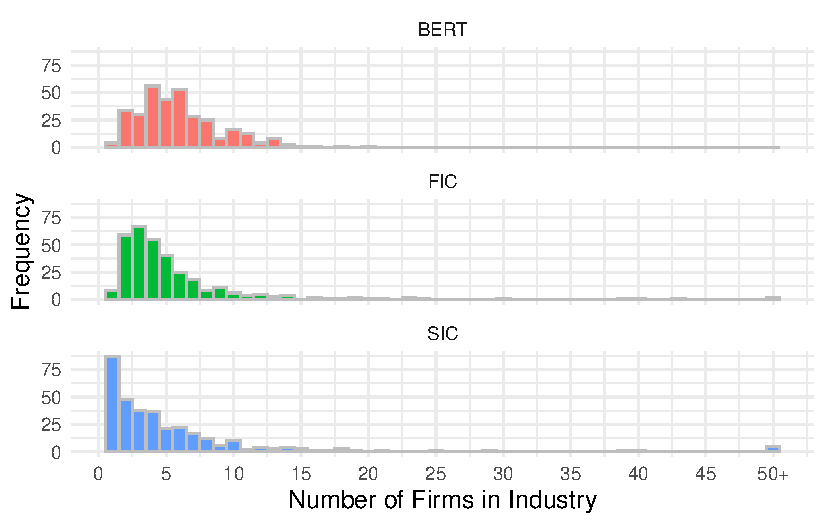
\includegraphics{ProjectEcoDataScience_files/figure-pdf/fig-1-1.pdf}

}

\caption{\label{fig-1}Density Function of the Distance}

\end{figure}%

\section{Estimation Strategy}\label{estimation-strategy}

We test H3 using multivariate regression techniques. In all the
specifications we use the Normalized Distance which we defined above as
the independent variable. In the first specification we employ for
measuring the firm performance the sales growth as our dependent
variable like Cucculelli \& Bettinelli (2015). We utilize our second
dataset and remove all observations with zero values for the market
value and the total assets. Furthermore, we use the z-score to drop
extreme growth rates. For a more detailed discussion of this step see
Appendix C. In the second specification we use the growth of Tobin's Q
as described by Desyllas et al. (2022). The third dataset is used for
this specification. In both specifications we control for firm size in
the first specification with the logarithm of the market value and in
the second with the logarithm of the total assets (Dang, Li, and Yang
2018). In the first specification we use the interaction term of the
year and our BERTScore industry classification as fixed effect. We
utilize the interaction term of the year and the industry because this
captures possible heterogeneous effects of the industry classification
between different years. In the second specification we only use
industry fixed effects. In the robustness check we use the SIC codes
instead of our BERTScore industry classification. We do not control for
economical and political environment as White et al. (2022) suggest
since all of our companies are U.S. based.

\section{Results and Discussion}\label{results-and-discussion}

\subsection{Comparison}\label{comparison}

Our study builds on the idea of Hoberg \& Phillips (2016) to utilize
text data from 10-K filings to classify companies based on their product
similarity into dynamic industries. They achieve this through the
parsing of the product descriptions provided by Item 1 of firms 10-K
filings and creating word vectors. Specifically, the authors identify
and exclude proper nouns, which include common words and geographic
locations. They then create word vectors for each firm and year, which
enables the measurement of product similarity over time. They perform
two steps to create the FIC. Firstly, a hierarchical agglomerative
clustering algorithm is employed to cluster companies based on their
similarity and maximize ex-post within cluster similarity. This enables
a classification with any number of clusters. In the second step, the
authors compute aggregated word vectors for each industry. These vectors
now represent the industries. Subsequently, the similarity between
industries and firms is calculated for each of the following years. From
the second year onwards, firms are classified according to the industry
with which they are most similar. Our approach differs in two ways:
Firstly, in contrast to the TNIC and FIC, which employ word-to-vec, our
approach utilises BERT to represent text, which allows us to capture the
context of words. Accordingly, the BERTScore is employed instead of the
cosine similarity as our similarity measure. Secondly, our analysis is
focused on the description of the BM rather than on the product
descriptions. Nevertheless, in the following subsection, the BERTScore
industry classification is compared with the FIC and the SIC.

We employ the first dataset for the BERTScore industry classification
and the comparison. The SIC codes come from the SEC website\footnote{The
  list can be found here:
  https://www.sec.gov/search-filings/standard-industrial-classification-sic-code-list.}.
For the FIC we have utilized the similarity scores provided by
Hoberg-Phillips Data Library\footnote{For the database see:
  https://hobergphillips.tuck.dartmouth.edu.}. The data consists of the
gvkeys of two companies, the year and the cosine similarity between
these two companies. In order to ensure comparability, only companies
present in both the present study's dataset and that provided by the
authors are included in the analysis. Because we use CIKs and accession
numbers to identify firms and filings, and the fact that the data
library employs Compustat's gvkeys, the matching of CIKs with gvkeys
inevitably results in the loss of some observations. Ultimately, for the
comparison the clustering algorithm was applied to 1,958 of the 3,246
firms in our sample for the year 2017. In our dataset, companies are
from 320 different SIC codes. Therefore, for the comparison the number
of industries chosen for our industry classification and the FIC is 320.

Figure 2 compares the distribution of industry size for the BERTScore
classification, the FIC and the SIC. Both the BERTScore classification
and the FIC show a similar distribution, displaying a leftward skew with
the majority of industries comprising fewer than ten firms. The SIC
shows as well a left skewed distribution but with most industries only
containing one company. The distribution of the FIC is steeper than the
one of the BERTScore classification. It is notable that the largest
industry in the BERTScore classification comprises only 20 companies,
whereas the FIC and SIC contain industries with a greater number of
firms, with some exceeding 50. This suggests that the BERTScore
classification groups small to medium-sized industries, comprising
between two and fourteen firms per industry, with fewer large
industries. The FIC also comprises mostly of small to medium-sized
industries, with a few larger ones. Despite these minor differences,
this supports H1. The degree of homogeneity between the BERTScore
classification and the FIC is 0.63, while the completeness is 0.6. This
demonstrates only a medium degree of overlap between the two
classifications. The Adjusted Rand Index (ARI) (Hubert and Arabie 1985)
is situated at 0.0002, which is close to zero, indicating that the
overlap might be random. These findings do not provide support for H2.

In order to use our BERTScore industry classification in our estimation,
we classify all 3,246 companies from the year 2017 as described above.
Since we use BERT and do not have word vectors for each industry, our
methodology differs in the second step from Hoberg \& Phillips (2016).
We assign the remaining companies of which we do not have data for the
year 2017 to the industry of the company which are already classified
and which they are most similar to.

\begin{figure}

\centering{

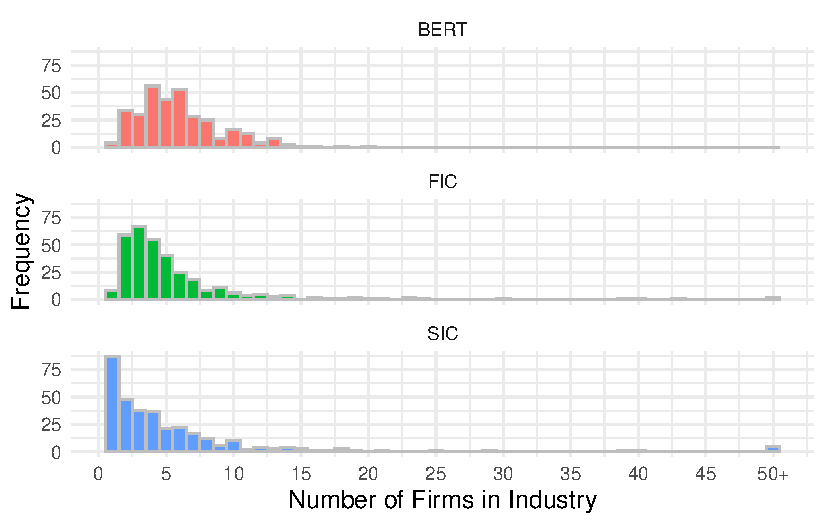
\includegraphics{ProjectEcoDataScience_files/figure-pdf/fig-2-1.pdf}

}

\caption{\label{fig-2}Distribution Comparison between BERT
Classification, FIC and SIC}

\end{figure}%

\subsection{Results}\label{results}

\begin{table}[!htbp] \centering 
  \caption{Regression Results} 
  \label{} 
\begin{tabular}{@{\extracolsep{5pt}}lcccc} 
\\[-1.8ex]\hline 
\hline \\[-1.8ex] 
 & \multicolumn{4}{c}{\textit{Dependent variable:}} \\ 
\cline{2-5} 
\\[-1.8ex] & \multicolumn{2}{c}{Sales Growth} & \multicolumn{2}{c}{Tobin's Q Growth} \\ 
\\[-1.8ex] & (1) & (2) & (3) & (4)\\ 
\hline \\[-1.8ex] 
 Normalized Distance & 0.289$^{***}$ & 0.292$^{***}$ & $-$0.008$^{***}$ & $-$0.008$^{***}$ \\ 
  & (0.110) & (0.110) & (0.001) & (0.001) \\ 
  & & & & \\ 
 log(Market Value) & $-$1.014 &  &  &  \\ 
  & (0.921) &  &  &  \\ 
  & & & & \\ 
 log(Assets) &  & $-$2.155$^{**}$ &  &  \\ 
  &  & (0.927) &  &  \\ 
  & & & & \\ 
 log(MeanAssets) &  &  & 0.0003 &  \\ 
  &  &  & (0.010) &  \\ 
  & & & & \\ 
 log(MeanMV) &  &  &  & 0.023$^{**}$ \\ 
  &  &  &  & (0.011) \\ 
  & & & & \\ 
 TimeDiff &  &  & 0.056$^{***}$ & 0.051$^{***}$ \\ 
  &  &  & (0.016) & (0.016) \\ 
  & & & & \\ 
\hline \\[-1.8ex] 
Industry x Year Fixed Effects & Yes & Yes & No & No \\ 
Industry Fixed Effects & No & No & Yes & Yes \\ 
Observations & 12,155 & 12,155 & 3,341 & 3,341 \\ 
R$^{2}$ & 0.248 & 0.248 & 0.193 & 0.194 \\ 
Residual Std. Error & 222.602 (df = 9914) & 222.555 (df = 9914) & 1.327 (df = 3013) & 1.326 (df = 3013) \\ 
\hline 
\hline \\[-1.8ex] 
\textit{Note:}  & \multicolumn{4}{r}{$^{*}$p$<$0.1; $^{**}$p$<$0.05; $^{***}$p$<$0.01} \\ 
\end{tabular} 
\end{table}

\newpage{}

Table 3 presents the four regressions related to hypothesis H3. The
theory posits that changes in the business model are positively
correlated with firm performance. As previously described, this
relationship is examined using sales growth and Tobin's Q growth as
performance indicators. The first two regressions focus on sales growth
as the dependent variable. Both regressions yield similar results when
considering the key parameter relevant to our hypothesis. As anticipated
from our hypothesis formulation, we expected a positive relationship
between business model changes and performance. This is confirmed in
both regressions, providing support for H3. Importantly, this finding
holds regardless of whether we include the market value or total capital
(logarithmically transformed) as a control variable.

Both control variables reduce the effect on sales growth, with market
value being insignificant and having a smaller impact. While this result
is not particularly relevant for the first two regressions, it suggests
a direction in which Tobin's Q might change in response to business
model adjustments. Since Tobin's Q is defined as market value divided by
total capital, the relationship should mirror the patterns observed with
market value and total capital in the previous regressions. This effect
is observed in both regressions where Tobin's Q is the dependent
variable. In regression (4), both control variables are significant,
while in regression (3), only TimeDiff shows significance.

In summary, the findings indicate that business model adaptation has a
significant impact on firm performance. Specifically, business model
changes have a positive effect on operational metrics such as sales
growth, which can be viewed as a positive outcome. However, the stock
market does not respond as favorably to such changes. Tobin's Q ratio
decreases when companies adjust their business models, meaning the ratio
of market value to total capital declines. This effect is not
necessarily problematic, as market value is influenced by stock trading,
which incorporates subjective evaluations that are reflected in this
metric.

\subsection{Robustness Checks}\label{robustness-checks}

To check the validity and reliability of this study, we conduct a series
of robustness checks, illustrating alternative models. We do not
logarithmize revenue growth and normalized distance. Revenue growth can
assume negative values and is a relative measure. The normalized
distance is also a relative measure, and the distance itself is
characterized by a norm distribution (according to Figure 1).
Logarithmization is therefore not necessary. The use of market value and
total assets as control variables makes it possible to control for the
size of the company, which results on the one hand from supply and
demand on the capital market, and on the other hand from the actual book
value of the company. The correlation between these two variables is
approximately 0.5. In Table 4, we perform a regression using SIC codes
instead of the industry classification based on BERTScores as fixed
effects.

\begin{table}[!htbp] \centering 
  \caption{Robustness Check} 
  \label{} 
\begin{tabular}{@{\extracolsep{5pt}}lcccc} 
\\[-1.8ex]\hline 
\hline \\[-1.8ex] 
 & \multicolumn{4}{c}{\textit{Dependent variable:}} \\ 
\cline{2-5} 
\\[-1.8ex] & \multicolumn{2}{c}{Sales Growth} & \multicolumn{2}{c}{Tobin's Q Growth} \\ 
\\[-1.8ex] & (1) & (2) & (3) & (4)\\ 
\hline \\[-1.8ex] 
 Normalized Distance & 0.180 & 0.185 & $-$0.009$^{***}$ & $-$0.009$^{***}$ \\ 
  & (0.129) & (0.129) & (0.001) & (0.001) \\ 
  & & & & \\ 
 log(Market Value) & $-$4.112$^{***}$ &  &  &  \\ 
  & (1.010) &  &  &  \\ 
  & & & & \\ 
 log(Assets) &  & $-$5.157$^{***}$ &  &  \\ 
  &  & (0.965) &  &  \\ 
  & & & & \\ 
 log(MeanAssets) &  &  & 0.029$^{***}$ &  \\ 
  &  &  & (0.010) &  \\ 
  & & & & \\ 
 log(MeanMV) &  &  &  & 0.049$^{***}$ \\ 
  &  &  &  & (0.011) \\ 
  & & & & \\ 
 TimeDiff &  &  & 0.098$^{***}$ & 0.096$^{***}$ \\ 
  &  &  & (0.018) & (0.018) \\ 
  & & & & \\ 
\hline \\[-1.8ex] 
Industry x Year Fixed Effects & Yes & Yes & No & No \\ 
Industry Fixed Effects & No & No & Yes & Yes \\ 
Observations & 11,187 & 11,187 & 2,977 & 2,977 \\ 
R$^{2}$ & 0.139 & 0.140 & 0.131 & 0.134 \\ 
Residual Std. Error & 247.816 (df = 8805) & 247.647 (df = 8805) & 1.416 (df = 2624) & 1.414 (df = 2624) \\ 
\hline 
\hline \\[-1.8ex] 
\textit{Note:}  & \multicolumn{4}{r}{$^{*}$p$<$0.1; $^{**}$p$<$0.05; $^{***}$p$<$0.01} \\ 
\end{tabular} 
\end{table}

The number of observations decreases due to missing SIC codes for
non-surviving companies. As a result Table 4 rather tend to contain a
survivalship bias. Furthermore, the coefficients for sales growth are
not significant anymore, the standard errors of the coefficients are
increasing despite lower coefficient values. The value for \(R^2\) also
decreases for every model. The number of observations decreases due to
missing SIC codes for non-surviving companies. As a result, the models
in Table 4 contain a survivalship bias. In addition, the coefficients
for sales growth are no longer significant, the standard errors of the
coefficients increase despite lower coefficient values. The value for
\(R^2\) also decreases for each model. As a result, BERT-based industry
classifications as fixed effects tend to contain industry-based
endogenous effects and thus increase the validity of the model and the
informative value of the model.

\newpage{}

\subsection{Discussion}\label{discussion}

This study represents an innovative extension of Hoberg \& Phillips
(2016) work regarding their approach. While using the BERT-Score compels
us to shorten and condense the descriptions of business models, it
integrates semantics into the similarity calculation. As a result, the
entire text is considered, which appears to provide better informational
value compared to solely relying on frequently occurring nouns. However,
one potential critique of BERT is its limited ability to recognize
implicit and subtle meanings (1). The approach can only process the
textual descriptions. In this work, we exclusively examine business
models that provide little insight into current success in practice.
Notably, there are no clear objective statements, as with many key
financial indicators, that can be categorized as positive or
negative.(3) A positive description of negative aspects is unlikely in
this context, which justifies the use of the BERT-Score.

The use of BERT, and the consequent limitation regarding text length,
posed additional challenges in this research. In recent years, the
possibilities for utilizing AI have grown immensely. With the help of
GitHub Actions, we were able to obtain suitable access to Gemini. This
brings us to the most critical point of this work. This approach raises
transparency issues for the results. The system does not provide
explainable intelligence, meaning we cannot fully verify how exactly the
texts are generated. Our only option is to delegate the task and trust
the results' accuracy.

Nevertheless, we consider the current approach as the best possible
solution for condensing our business models. On the one hand, the
extracted texts do not follow the same structure across companies, and
on the other, cutting the business models arbitrarily poses too great a
risk. Losing up to 90\% of the content would be unacceptable in this
case, and due to structural differences, this becomes impossible beyond
certain key points. Moreover, the summaries generated by GPT have
sometimes been perceived as better than models specifically designed for
this purpose (2). A significant portion of this work involved data
collection, which proved to be a major challenge. Due to the lack of
access to Compustat, commonly used in financial studies and for
SEC-related information, we had to rely on extensive research. Various
approaches had to be abandoned as they failed to meet expectations.
Nonetheless, we were able to complete our work, though with a few
compromises regarding data volume.

A significant portion of this work involved data collection, which
proved to be a major challenge. Due to the lack of access to Compustat,
commonly used in financial studies and for SEC-related information, we
had to rely on extensive research. Various approaches had to be
abandoned as they failed to meet expectations. Nonetheless, we were able
to complete our work, though with a few compromises regarding data
volume.

In conclusion, the findings of our study suggest that Business Model
Innovation (BMI) is associated with improved performance, specifically
in terms of operating revenue. However, we can only report a correlation
rather than a causal effect, as the complexity of organizations is
substantial, and our dataset does not allow for definitive conclusions
regarding causality. Nonetheless, this study can be viewed as a
continuation of the approach by Hoberg et al., and the examination of
BMI's impact on performance could be further explored in future studies,
offering valuable extensions to this research.

\section{Conclusion}\label{conclusion}

\begin{itemize}
\tightlist
\item
  Summary of Findings: Summarize the main findings, emphasizing the
  replication and your original contributions.
\item
  Contribution to the Literature: Restate how your paper advances the
  field, particularly in light of the replication. This is where you can
  argue for the robustness of your findings and their implications.
\item
  Policy Implications: If applicable, discuss any policy implications of
  your results, grounding them in the empirical evidence presented.
\item
  Final Remarks: Conclude with any thoughts on future research or
  unresolved questions that your study raises.
\end{itemize}

\section{Acknowledgement}\label{acknowledgement}

\begin{itemize}
\tightlist
\item
  Jonathan for IT Support
\item
  Prof.~Kranz for Repo
\item
  bw unicluster
\end{itemize}

\newpage{}

\section{References}\label{references}

\phantomsection\label{refs}
\begin{CSLReferences}{1}{0}
\bibitem[\citeproctext]{ref-clauss_measuring_2017}
Clauss, Thomas. 2017. {``Measuring Business Model Innovation:
Conceptualization, Scale Development, and Proof of Performance.''}
\emph{R\&D Management} 47 (3): 385--403.
\url{https://doi.org/10.1111/radm.12186}.

\bibitem[\citeproctext]{ref-cucculelli_business_2015}
Cucculelli, Marco, and Cristina Bettinelli. 2015. {``Business Models,
Intangibles and Firm Performance: Evidence on Corporate Entrepreneurship
from {Italian} Manufacturing {SMEs}.''} \emph{Small Business Economics}
45 (2): 329--50. \url{https://doi.org/10.1007/s11187-015-9631-7}.

\bibitem[\citeproctext]{ref-dang2018measuring}
Dang, Chongyu, Zhichuan Frank Li, and Chen Yang. 2018. {``Measuring Firm
Size in Empirical Corporate Finance.''} \emph{Journal of Banking \&
Finance} 86: 159--76.

\bibitem[\citeproctext]{ref-Desyllas2022}
Desyllas, Panos, Ammon Salter, and Oliver Alexy. 2022. {``The Breadth of
Business Model Reconfiguration and Firm Performance.''} \emph{Strategic
Organization} 20 (2): 231--69.
\url{https://doi.org/10.1177/1476127020955138}.

\bibitem[\citeproctext]{ref-foss_fifteen_2017}
Foss, Nicolai J., and Tina Saebi. 2017. {``Fifteen {Years} of {Research}
on {Business} {Model} {Innovation}: {How} {Far} {Have} {We} {Come}, and
{Where} {Should} {We} {Go}?''} \emph{Journal of Management} 43 (1):
200--227. \url{https://doi.org/10.1177/0149206316675927}.

\bibitem[\citeproctext]{ref-hoberg_text-based_2016}
Hoberg, Gerard, and Gordon Phillips. 2016. {``Text-{Based} {Network}
{Industries} and {Endogenous} {Product} {Differentiation}.''}
\emph{Journal of Political Economy} 124 (5): 1423--65.
\url{https://doi.org/10.1086/688176}.

\bibitem[\citeproctext]{ref-huang_review_2023}
Huang, WenJun, and Takeyasu Ichikohji. 2023. {``A Review and Analysis of
the Business Model Innovation Literature.''} \emph{Heliyon} 9 (7):
e17895. \url{https://doi.org/10.1016/j.heliyon.2023.e17895}.

\bibitem[\citeproctext]{ref-hubert_comparing_1985}
Hubert, Lawrence, and Phipps Arabie. 1985. {``Comparing Partitions.''}
\emph{Journal of Classification} 2 (1): 193--218.
\url{https://doi.org/10.1007/BF01908075}.

\bibitem[\citeproctext]{ref-latifi_business_2021}
Latifi, Mohammad-Ali, Shahrokh Nikou, and Harry Bouwman. 2021.
{``Business Model Innovation and Firm Performance: {Exploring} Causal
Mechanisms in {SMEs}.''} \emph{Technovation} 107 (September): 102274.
\url{https://doi.org/10.1016/j.technovation.2021.102274}.

\bibitem[\citeproctext]{ref-lee_business_2014}
Lee, Jihwan, and Yoo S. Hong. 2014. {``Business {Model} {Mining}:
{Analyzing} a {Firm}'s {Business} {Model} with {Text} {Mining} of
{Annual} {Report}.''} \emph{Industrial Engineering and Management
Systems} 13 (4): 432--41.
\url{https://doi.org/10.7232/iems.2014.13.4.432}.

\bibitem[\citeproctext]{ref-pucihar_drivers_2019}
Pucihar, Andreja, Gregor Lenart, Mirjana Kljajić Borštnar, Doroteja
Vidmar, and Marjeta Marolt. 2019. {``Drivers and {Outcomes} of
{Business} {Model} {Innovation}---{Micro}, {Small} and {Medium}-{Sized}
{Enterprises} {Perspective}.''} \emph{Sustainability} 11 (2): 344.
\url{https://doi.org/10.3390/su11020344}.

\bibitem[\citeproctext]{ref-sec_investor_2024}
SEC. 2024. {``Investor {Bulletin}: {How} to {Read} a 10-{K}.''}
\url{https://www.sec.gov/files/reada10k.pdf}.

\bibitem[\citeproctext]{ref-spieth_business_2016}
Spieth, Patrick, and Sabrina Schneider. 2016. {``Business Model
Innovativeness: Designing a Formative Measure for Business Model
Innovation.''} \emph{Journal of Business Economics} 86 (6): 671--96.
\url{https://doi.org/10.1007/s11573-015-0794-0}.

\bibitem[\citeproctext]{ref-teece_business_2018}
Teece, David J. 2018. {``Business Models and Dynamic Capabilities.''}
\emph{Long Range Planning} 51 (1): 40--49.
\url{https://doi.org/10.1016/j.lrp.2017.06.007}.

\bibitem[\citeproctext]{ref-vaswani2017attention}
Vaswani, Ashish, Noam Shazeer, Niki Parmar, Jakob Uszkoreit, Llion
Jones, Aidan N Gomez, Lukasz Kaiser, and Illia Polosukhin. 2017.
{``Attention Is All You Need.(nips), 2017.''} \emph{arXiv Preprint
arXiv:1706.03762} 10: S0140525X16001837.

\bibitem[\citeproctext]{ref-white_exploring_2022}
White, Joshua V., Erik Markin, David Marshall, and Vishal K. Gupta.
2022. {``Exploring the Boundaries of Business Model Innovation and Firm
Performance: {A} Meta-Analysis.''} \emph{Long Range Planning} 55 (5):
102242. \url{https://doi.org/10.1016/j.lrp.2022.102242}.

\bibitem[\citeproctext]{ref-zott_fit_2008}
Zott, Christoph, and Raphael Amit. 2008. {``The Fit Between Product
Market Strategy and Business Model: Implications for Firm
Performance.''} \emph{Strategic Management Journal} 29 (1): 1--26.
\url{https://doi.org/10.1002/smj.642}.

\end{CSLReferences}

\newpage{}

\section{Appendix}\label{appendix}

\subsection{Appendix A}\label{appendix-a}

We used following prompt: ``Summarize the business model from the
following text. Answer with a continuous text and with five hundred
twelve tokens at max. Set your focus on sources of revenue, the intended
customer base, products, distribution channels and details of financing.
Use only information from the following the text''.\footnote{The
  spelling error in the last sentence of the prompt was found after
  processing Item 1. After evaluating the summaries, this error did not
  cause any issues.} ``intended customer base'' and ``product'' refer to
the value offering, ``distribution channels'' refers to the value
architecture, and ``sources of revenue'' and ``details of financing''
refer to the revenue model. The term `tokens' was used deliberately in
preference to `words', given that the number of tokens and the number of
words in a text may vary depending on the tokeniser. This way, we wanted
to ensure that the whole summary is used by the BERT model.

\begin{table}[H]
\centering
\caption{Descriptive Statistics of Number of Words of our Summaries}
\centering
\resizebox{\ifdim\width>\linewidth\linewidth\else\width\fi}{!}{
\begin{tabular}[t]{rrrrrrrr}
\toprule
Report-for Year & Average Word Count & Standard Deviation & Minimum & 25th Percentile & Median & 75th Percentile & Maximum\\
\midrule
2016 & 355 & 156 & 116 & 273 & 331 & 409 & 5377\\
2017 & 356 & 154 & 117 & 274 & 331 & 407 & 5951\\
2018 & 350 & 109 & 31 & 275 & 330 & 404 & 1057\\
2019 & 358 & 186 & 56 & 276 & 333 & 407 & 6273\\
2020 & 367 & 214 & 56 & 276 & 337 & 422 & 6872\\
\addlinespace
2021 & 370 & 159 & 76 & 281 & 344 & 432 & 5559\\
2022 & 371 & 161 & 138 & 283 & 345 & 425 & 6361\\
2023 & 366 & 207 & 150 & 275 & 333 & 419 & 5154\\
\bottomrule
\multicolumn{8}{l}{\rule{0pt}{1em}\textit{Note: }}\\
\multicolumn{8}{l}{\rule{0pt}{1em}All 21,417 original filings were considered.}\\
\end{tabular}}
\end{table}

\subsection{Appendix B}\label{appendix-b}

list of summaries we checked

\subsection{Appendix C}\label{appendix-c}

explain, why we drop some data points.

show regression without dropped data points

\begin{figure}

\centering{

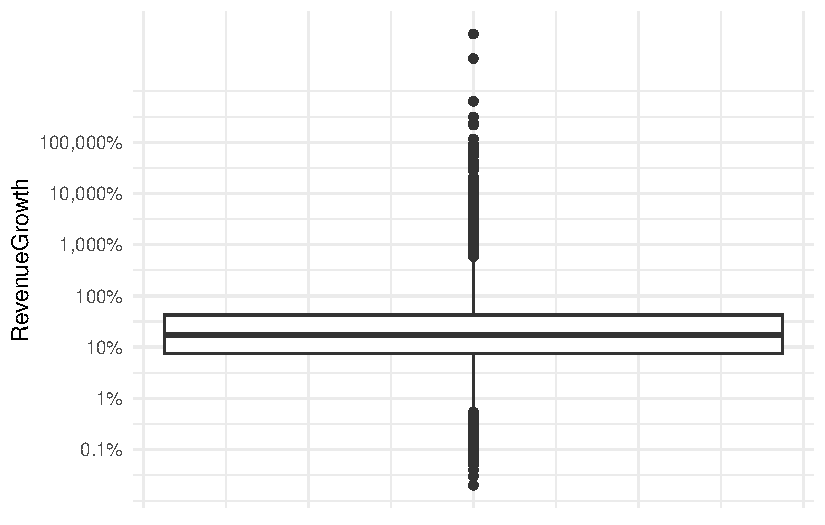
\includegraphics{ProjectEcoDataScience_files/figure-pdf/fig-3-1.pdf}

}

\caption{\label{fig-3}Distribution of the Sales Growth}

\end{figure}%

\begin{table}[!htbp] \centering 
  \caption{Regression Results} 
  \label{} 
\begin{tabular}{@{\extracolsep{5pt}}lcc} 
\\[-1.8ex]\hline 
\hline \\[-1.8ex] 
 & \multicolumn{2}{c}{\textit{Dependent variable:}} \\ 
\cline{2-3} 
\\[-1.8ex] & \multicolumn{2}{c}{Sales Growth} \\ 
\\[-1.8ex] & (1) & (2)\\ 
\hline \\[-1.8ex] 
 Normalized Distance & 41.999 & 41.800 \\ 
  & (50.080) & (50.087) \\ 
  & & \\ 
 log(Market Value) & 581.110 &  \\ 
  & (420.543) &  \\ 
  & & \\ 
 log(Assets) &  & 330.692 \\ 
  &  & (423.289) \\ 
  & & \\ 
\hline \\[-1.8ex] 
Industry x Year Fixed Effects & Yes & Yes \\ 
Observations & 12,155 & 12,155 \\ 
R$^{2}$ & 0.458 & 0.458 \\ 
Residual Std. Error (df = 9914) & 101,623.500 & 101,630.200 \\ 
\hline 
\hline \\[-1.8ex] 
\textit{Note:}  & \multicolumn{2}{r}{$^{*}$p$<$0.1; $^{**}$p$<$0.05; $^{***}$p$<$0.01} \\ 
\end{tabular} 
\end{table}



\end{document}
